\section{Conjuntos de datos}\label{sec:datasets}

Para desarrollar los experimentos, se conformaron 3 conjuntos de datos con segmentos correspondientes a vocalizaciones de especies de murciélagos, aves e insectos.
En las tablas~\ref{table:bats-dataset},~\ref{table:birds-dataset} y~\ref{table:insects-dataset} se describen las especies que componen cada uno de estos conjuntos.
Un cuarto conjunto de datos fue constituido a partir de la unión de los anteriores.
Todos los segmentos se extrajeron de forma manual a partir de grabaciones de mayor duración.

La diversidad de sonidos que pueden producir los individuos de una misma especie, hace que en la clasificación de los segmentos no baste con recoger simplemente el nombre de la especie de la que proceden.
Por tal razón, se empleó además un identificador para distinguir entre tipos de vocalizaciones diferentes aun cuando estas pudieran provenir de individuos pertenecientes a la misma especie.
De esta forma es posible evaluar mejor los resultados de los algoritmos abordados en este trabajo;
pudiendo distinguirse así entre situaciones en que el algoritmo separó incorrectamente dos clusters de aquellas en que dicha acción tenía sentido por tratarse de tipos de vocalizaciones diferentes.

\section{Resultados}\label{sec:results}

Para la experimentación se emplearon todas las combinaciones de 14 de las características mencionadas en este trabajo:

\begin{multicols}{2}
    \begin{enumerate}
        \item \hyperref[subsec:log-attackTime]{Log-Attack Time}
        \item \hyperref[subsec:audioPower]{Audio Power}
        \item \hyperref[subsec:temporalCentroid]{Temporal Centroid}
        \item \hyperref[subsec:effectiveDuration]{Effective Duration}
        \item \hyperref[subsec:auto-correlation]{Auto-correlation}
        \item \hyperref[subsec:zeroCrossingRate]{Zero Crossing Rate}
        \item \hyperref[itemize:basic-spectral-features]{Frecuencia pico}
        \item \hyperref[itemize:basic-spectral-features]{Frecuencia máxima}
        \item \hyperref[itemize:basic-spectral-features]{Frecuencia mínima}
        \item \hyperref[itemize:basic-spectral-features]{Bandwidth}
        \item \hyperref[subsubsec:spectralCentroid]{Spectral Centroid}
        \item \hyperref[subsubsec:spectrallRollOff]{Spectral Roll-off}
        \item \hyperref[subsec:spectralFlux]{Spectral Flux}
        \item \hyperref[sec:MFCC]{MFCC}
    \end{enumerate}
\end{multicols}

En el caso de las características 2 y 5 se consideró la suma de todos los elementos de dichos vectores.
Para las numeradas entre 7 y 13, se consideró el promedio de los coeficientes correspondientes a las posiciones inicial, final, central, de valor máximo y de máxima amplitud del espectro.
Para los MFCC se empleó el vector obtenido al promediar cada uno de los coeficientes en el tiempo.

Los valores de algunas de las medidas de evaluación, aplicadas a los resultados obtenidos, aparecen resumidos en el Apéndice~\ref{ch:experimentsResults}.

En las figuras~\ref{img:bats},~\ref{img:birds},~\ref{img:insects} y~\ref{img:all} se resume la evaluación de los resultados aplicando el medidor \textit{Adjusted Rand Index};
para tres de estas combinaciones: la conformada por todas las características de la 1 a la 13 (nombradas características \textit{descriptivas}), la que solamente incluye los MFCC, y la que incluye a las 14 características.

\begin{figure}[!h]
    \centering
    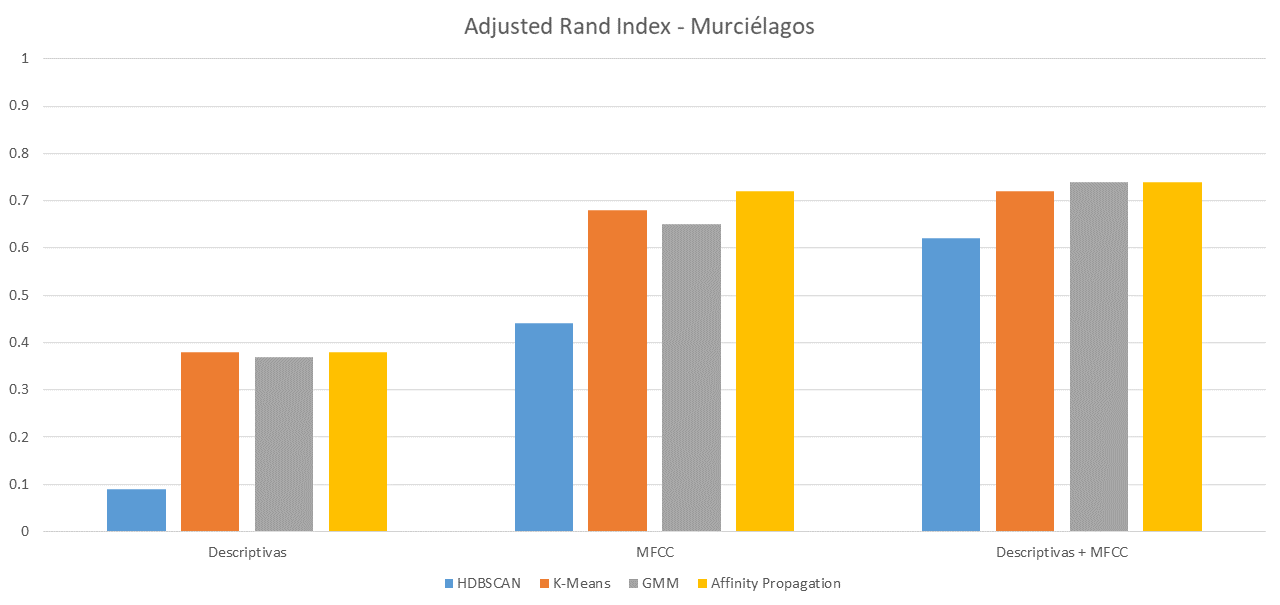
\includegraphics[width=\textwidth]{bats.png}
    \caption{Valores del criterio \textit{Adjusted Rand Index} para el conjunto de datos de murciélagos, en correspondencia con las características y el algoritmo de clustering empleado.}
    \label{img:bats}
\end{figure}

\begin{figure}[!h]
    \centering
    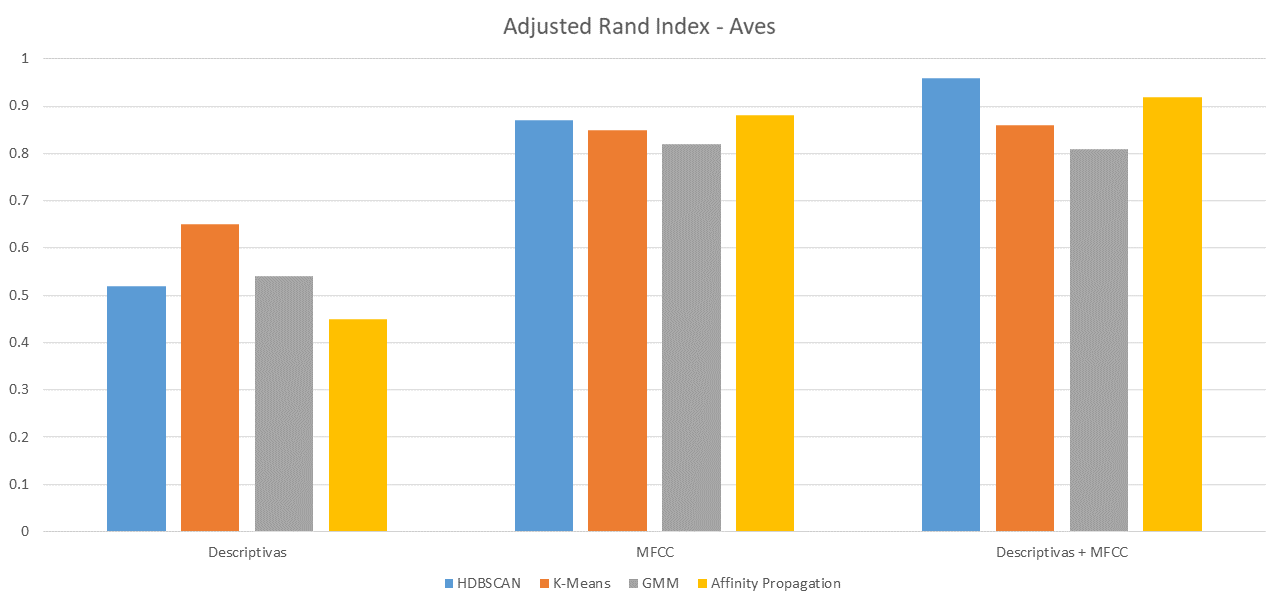
\includegraphics[width=\textwidth]{birds.png}
    \caption{Valores del criterio \textit{Adjusted Rand Index} para el conjunto de datos de aves, en correspondencia con las características y el algoritmo de clustering empleado.}
    \label{img:birds}
\end{figure}

\begin{figure}[!h]
    \centering
    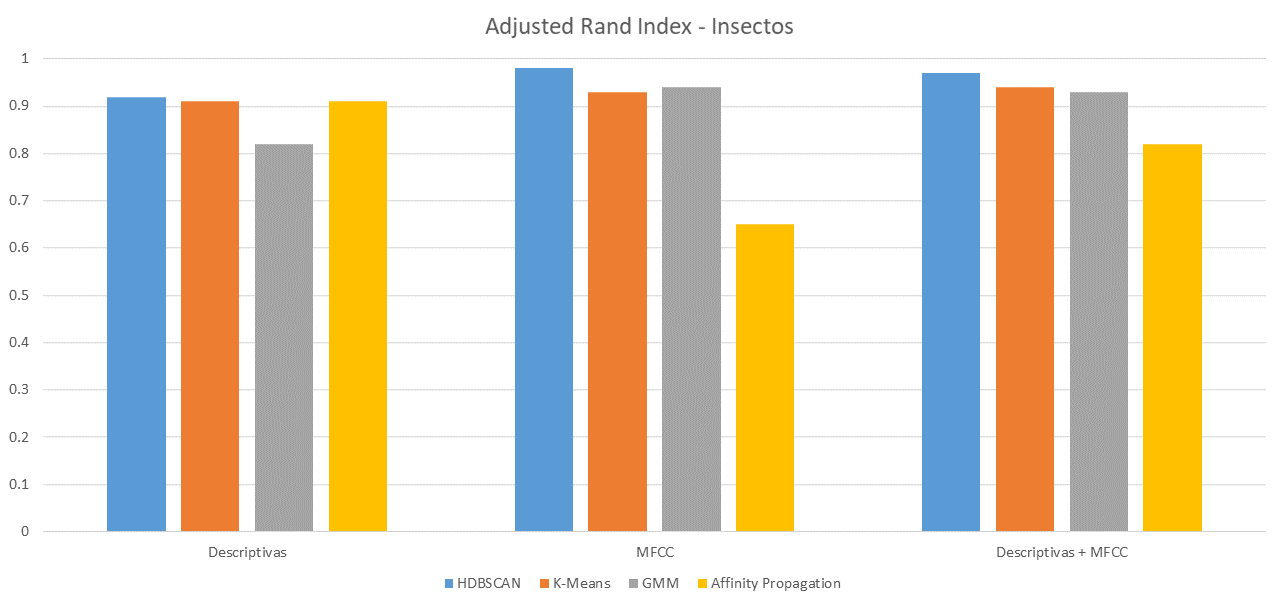
\includegraphics[width=\textwidth]{insects.png}
    \caption{Valores del criterio \textit{Adjusted Rand Index} para el conjunto de datos de insectos, en correspondencia con las características y el algoritmo de clustering empleado.}
    \label{img:insects}
\end{figure}

\begin{figure}[!h]
    \centering
    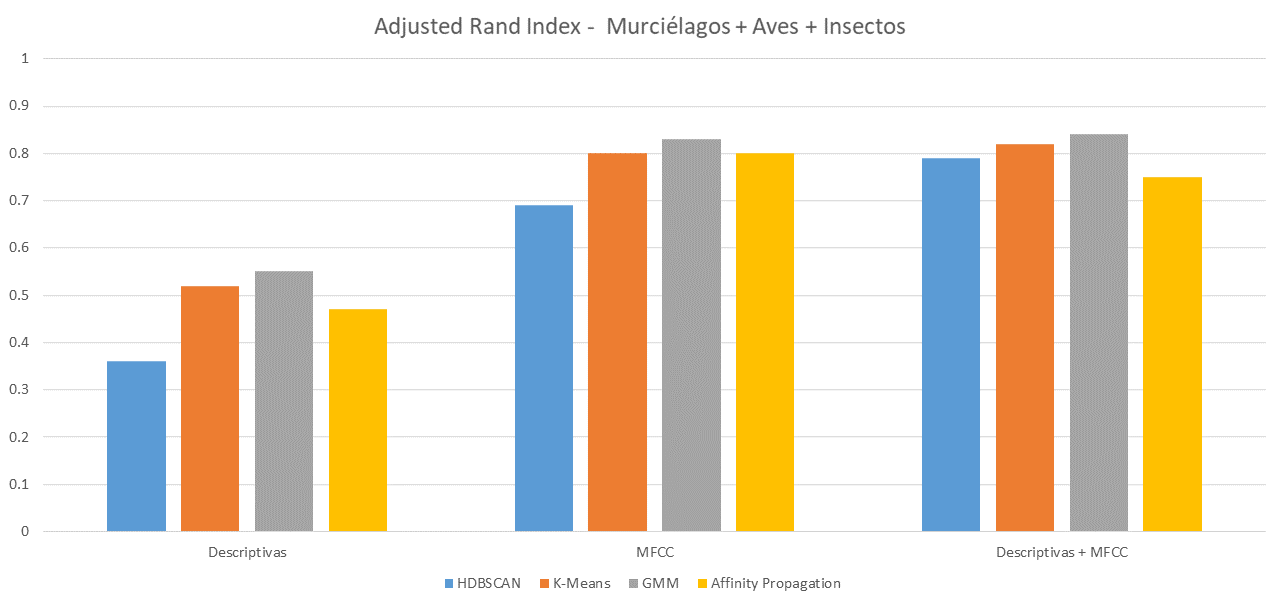
\includegraphics[width=\textwidth]{all.png}
    \caption{Valores del criterio \textit{Adjusted Rand Index} para el conjunto de datos conformado por la unión de los de murciélagos, aves e insectos, en correspondencia con las características y el algoritmo de clustering empleado.}
    \label{img:all}
\end{figure}

Se puede observar que en general los resultados son mucho mejores cuando los MFCC se encuentran presentes en las características utilizadas.
Si bien añadir características adicionales a dicho vector contribuye en la mayoría de los casos a incrementar la calidad del resultado se incrementa, el valor en que lo hace no es demasiado significativo.

Puede apreciarse además que la selección del algoritmo no pesa tanto sobre la evaluación del resultado como lo hace la del conjunto de características.
